\newpage
\phantomsection
\let\cleardoublepage\clearpage
\part{Производственные и обрабатывающие отрасли}
\chapter{Технология продовольственных продуктов}

{\bfseries ҒТАМР 65.63.03}
\hfill {\bfseries \href{https://doi.org/10.58805/kazutb.v.2.23-282}{https://doi.org/10.58805/kazutb.v.2.23-282}}

\sectionwithauthors{Ф.Т. Диханбаева , Г.Е. Есиркеп, Г.С. Жунусова, Ж.Нармандах, Б.Калемшарив}{ҚЫМЫЗ ӨНДІРІСІНДЕ ТАБИҒИ ҚОСПАЛАРДЫ ПАЙДАЛАНУ}

\begin{center}
{\bfseries \textsuperscript{1}Ф.Т. Диханбаева\envelope, \textsuperscript{2}Г.Е. Есиркеп, \textsuperscript{2}Г.С. Жунусова, \textsuperscript{2}Ж.Нармандах, \textsuperscript{3}Б.Калемшарив}

\textsuperscript{1}Алматы технологиялық университеті, Алматы, Қазақстан,

\textsuperscript{2}Қ. Құлажанов атындағы Қазақ технология және бизнес
университеті, Астана, Қазақстан,

\textsuperscript{3}С. Сейфуллин атындағы Қазақ агротехникалық зерттеу
университеті, Астана, Қазақстан

\envelope Корреспондент-автор: fatima6363@mail.ru
\end{center}

Берілген мақалада зерттеудің негізгі мақсаты -- адам денсаулығына
пайдалы әсер ететін бие сүті және қымызды өндірудің дәстүрлі әдісін
қолдана отырып қара өрік қосылған қымызды алудың сапасы мен
технологиясын жаңарту, жаңа құрамды бие сүтінен қара өрік ұнтағы
араласқан үлгілеріне арналған ғылыми негізделген рецепттерді құрастырып,
пробиотикалық ашытылған бие сүтін дайындау болып табылады.

Соңғы уақытта бие сүтін өндіруге қызығушылық арта түсті, себебі оның
құрамында көптеген құнды қоректік заттар бар, сонымен қатар, денсаулықты
жақсартатын пайдасы зор. Адам мен бие сүтіндегі Ca-P қатынасы сиыр
сүтіндегі қатынаспен салыстырғанда Ca-ны сіңіру үшін қолайлы екені
көрсетілді.

Зерттеу кезеңі нәтижесінде пробиотикалық ашытылған бие сүті, қара өрік
ұнтағы, жоғары талшықты және пробиотикалық ашытылған бие сүті
дайындалып, қара өрік қосылған қымызды дайындау технологиясы үлгілік
сызбасы әзірленді.

Осылайша, қымыз өнімінің технологиясын әзірлеу жоғарғы тұтынушылық
қасиеттері бар функционалды тамақ өнімдерін құрудың жаңа және
перспективалы тәсілі болып табылады.

{\bfseries Түйін сөздер:} сүт, бие сүті, сиыр сүті, ана сүті, қымыз, қара
өрік ұнтағы, функционалдық тамақ, пробиотикалық, пребиотикалық.

\begin{center}
{\large\bfseries ИСПОЛЬЗОВАНИЕ НАТУРАЛЬНЫХ ДОБАВОК В ПРОИЗВОДСТВЕ КУМЫСА}

{\bfseries \textsuperscript{1}Ф.Т. Диханбаева\envelope, \textsuperscript{2}Г.Е. Есиркеп, \textsuperscript{2}Г.С. Жунусова, \textsuperscript{2}Ж. Нармандах, \textsuperscript{3}Б. Калемшарив}

\textsuperscript{1}Алматинский технологический университет, Алматы,
Казахстан,

\textsuperscript{2}Казахский университет технологии и бизнеса им.
К.Кулажанова, Астана, Казахстан,

\textsuperscript{3}Казахский исследовательский аграрный университет им.
С. Сейфуллина, Астана, Казахстан,

e-mail: fatima6363@mail.ru
\end{center}

Основной целью исследования в данной статье является исследование
качества и разработка технологии напитка традиционным способом из
кошерного молока и кошерной сливы, благотворно влияющей на здоровье
человека, создание научно обоснованных рецептур, получение новых
композиций на основе кобыльего молока смешанных с порошком из сливы и
приготовление пробиотического ферментированного кобыльего молока.

В последнее время возрос интерес к производству кобыльего молока,
поскольку оно содержит множество ценных питательных веществ, обладающее
оздоровительными свойствами. Было показано, что соотношение Ca-P в
человеческом и кобыльем молоке более благоприятно для усвоения
организмом Ca, чем в коровьем молоке.

В результате исследовательской работы был разработан напиток из
кобыльего молока ферментированного пробиотиками, с использованием
сливового порошка и меда, и разработана технологическая схема
приготовления кошерного молока со сливой.

Таким образом, разработка технологии производства кумыса является новым
и перспективным направлением при создании функциональных продуктов
питания с высокими потребительскими свойствами.

{\bfseries Ключевые слова:} молоко, кобылье молоко, коровье молоко, грудное
молоко, кумыс, порошок чернослива, функциональная пища, пробиотик,
пребиотик.

\begin{center}
{\large\bfseries THE USE OF NATURAL ADDITIVES IN THE PRODUCTION OF KUMISS}

{\bfseries \textsuperscript{1}F.T. Dikhanbayeva\envelope, \textsuperscript{2}G.E. Esirkep, \textsuperscript{2}G.S. Zhunusova, \textsuperscript{2}Zh.Narmandakh, \textsuperscript{3}B. Kalemshariv}

\textsuperscript{1}Almaty Technological University, Almaty, Kazakhstan,

\textsuperscript{2}Kazakh University of Technology and Business named
after K. Kulajanov, Astana, Kazakhstan,

\textsuperscript{3}Kazakh Research Agrarian University named after S.
Seifullin, Astana, Kazakhstan,

e-mail: fatima6363@mail.ru
\end{center}

The main goal of the research in this article is to update the quality
and technology of producing kosher with plums using the traditional
method of producing mare\textquotesingle s milk and kosher, which has a
beneficial effect on human health, to create scientifically based
recipes for samples of new composition of mare\textquotesingle s milk
mixed with plum powder, and to prepare probiotic fermented
mare\textquotesingle s milk. is.

Recently, there has been an increased interest in the production of
mare\textquotesingle s milk, because it contains many valuable
nutrients, as well as health-improving properties. The Ca-P ratio in
human and mare\textquotesingle s milk has been shown to be more
favorable for Ca absorption than that in cow\textquotesingle s milk.

As a result of the research period, probiotic-fermented
mare\textquotesingle s milk, plum powder, high-fiber and
probiotic-fermented mare\textquotesingle s milk were prepared, and a
sample drawing of the technology of preparation of kosher with plum was
developed.

Thus, the development of kumif product technology is a new and promising
way to create functional food products with high consumer properties.

{\bfseries Keywords:} milk, mare\textquotesingle s milk,
cow\textquotesingle s milk, breast milk, koumiss, prune powder,
functional food, probiotic, prebiotic.

\begin{multicols}{2}
{\bfseries Кіріспе.} Сүт -- аналық сүтқоректілердің ұрпақтарының қоректенуі
үшін бөлетін сұйықтық. Сүтқоректілердің сүтінің құрамдас бөліктерінің
көпшілігі су, май, ақуыз, көмірсулар, минералды және дәруменді заттар
болып табылады. Бие сүті («саумал») -- физиологиялық, нәзік және жай
ассимиляцияланған биологиялық белсенді өнім {[}1{]}.

Бие сүті құрамында фосфолипидтер мен А дәруменінің жоғары болуына
байланысты қышқылға қарсы қасиетке ие. Бие сүтін өкпе ауруы бар, әсіресе
туберкулезбен ауыратын науқастарды емдеу үшін пайдалану Ресей мен
Моңғолия аумағында ұзақ уақыт бойы қолданылып келеді. Сонымен қатар,
кейбір зерттеулерде бие сүтін пайдалану арқылы анемия, нефрит, диарея,
гастрит және басқа ас қорыту ауруларымен күресу мүмкіндігі бар екендігін
хабарлады {[}1{]}.

Бие сүтінің құрамы адам сүтіне ұқсас және ол лактоферрин, лизоцим, ω-3
және ω-6 май қышқылдарының жоғары концентрациясының болуына байланысты
көптеген биологиялық функцияларды орындауға қабілетті болуы керек
{[}2{]}.

Бие сүтінің құрамында адам ағзасына қажетті 40-қа жуық биологиялық
компоненттер: аминқышқылдары, майлар, ферменттер (лизоцим, амилаза),
микроэлементтер (кальций, натрий, калий, фосфор, темір, магний, мыс,
йод, күкірт, кобальт, мырыш, бром) және дәрумендер (A, C, B1, B2, B6,
B12, E, каротиноид, фолий қышқылы) оңтайлы теңдестірілген пропорцияда
кездеседі. Бие сүті лактозаның -- 72,80 г/л, майдың -- 6,40 г/л және
ақуыздар 15,52 г/л, атап айтқанда казеиндердің -- 13,4 г/л жеткілікті
мөлшерімен сипатталады. Бие сүтінің емдік маңызы бүкіл Ресей мен Батыс
Азия аумағында аңызға айналған. Моңғол дәрігерлері бие сүтін созылмалы
жұқпалы ауруларды, бауыр және ойық жара ауруларын емдеу үшін пайдалануды
тәжірибеге айналдырған {[}3{]}.

Бие сүтінің құрамы ана сүтіне ұқсас және ол лактоферрин, лизоцим, ω-3
және ω-6 май қышқылдарының жоғары концентрациясының болуына байланысты
көптеген биологиялық функцияларды орындауға қабілетті {[}3{]}.

Бие сүтінің химиялық құрамы. Сүттің жалпы құрамы түрлер арасында
айтарлықтай өзгеретіні мойындалады, өйткені түтік бездерінің секрециясы
әрбір нақты түрдегі жаңа туған нәрестенің биологиялық процесінің
қажеттіліктерімен физиологиялық және құрылымдық түрде байланысты
{[}4{]}.

1.2-кесте бие, ана және сиыр сүтінің жалпы құрамын, 3 түрдің арасында
маңызды өзгерістер болған жерде салыстыруды көрсетеді. Бие сүтіндегі
лактозаның мөлшерін ана сүтімен салыстыруға болады, сонымен қатар, ол
сиыр сүтінен жоғары. Алайда, бие мен ана сүтінде сиыр сүтімен
салыстырғанда ақуыздар мен минералдардың деңгейі айтарлықтай төмен
(1-кестеде көрсетілген).
\end{multicols}

\begin{table}[H]
\caption*{1-кесте -- Бие, ана, сиыр сүттерінің химиялық құрамы мен энергетикалық құндылықтары}
\centering
\begin{tabular}{|l|l|l|l|}
\hline
Құрамдас бөліктер & Бие сүті & Ана сүті & Сиыр сүті \\ \hline
Май, \% & 0,5-2,0 & 3,5-4,0 & 3,5-3,9 \\ \hline
Ақуыз, \% & 1,5-2,8 & 0,9-1,7 & 3,1-3,8 \\ \hline
Лактоза, \% & 5,8-7,0 & 6,3-7,0 & 4,4-4,9 \\ \hline
Күл, \% & 0,3-0,5 & 0,2-0,3 & 0,7-0,8 \\ \hline
Энергетикалық құндылығы, ккал/кДж & 390-550 & 650-700 & 650-712 \\ \hline
\end{tabular}
\end{table}

\begin{multicols}{2}
Биенің уыз сүтіндегі казеин мен сарысу ақуызының арақатынасы төлдегеннен
кейін бірден 0,2:1 құрайды және ол бір апта ішінде 1,1:1-ге өзгереді.
Бие сүті салыстырмалы түрде лактозаға бай және оның көлемі лактация
уақытында ақырындап азаяды. Бие сүтінің майлылығы лактацияның
жоғарылауымен төмендейді, ал ірі қара сүті лактацияның 3 айынан кейін
белгілі минимумды көрсетеді және одан кейін жоғарылайды. Бие сүтінің
энергетикалық құрамы ана мен сиыр сүтіне қарағанда айтарлықтай төмен
болып келеді. Бие сүтінің басқа сүтқоректілермен салыстырғанда майы аз,
оның мәні небәрі 5 г/кг-дан төмен. Бие сүті күлі 0,3-0,5\% аралығында
және бұл көрсеткіш ішінара кальций мен фосфордың, ақуыздың төмен
мазмұнымен байланысты {[}5{]}.

\emph{Липидтер.} Бие сүтінің майы ана мен сиыр сүтімен салыстырғанда өте
төмен. Төлдегеннен кейін бірден уыз сүтіндегі майдың мөлшері орташа
есеппен 2,9\%, ал өтпелі сүт және қалыпты сүттің орташа мөлшері
сәйкесінше 2,1\% және 1,2\% құрады. Уыз сүті мен қалыпты бие сүті
арасында майдың құрамында айқын айырмашылықтар болған жоқ. Сүт липидтері
эмульсияланған түйіршіктер түрінде таралады және бие сүтінің май
түйіршіктерінің мөлшері шамамен 2-3 мкм құрайды. Уыз сүтіндегі сүт
майының глобулды қабығы бие сүті сияқты гликопротеинді жіптермен
қапталған, олардың ұсынылатын рөлі майдың қорытылуын күшейту үшін
липазаларды байланыстырады {[}5{]}.

\emph{Ақуыз.} Бие сүтінде сиыр сүтімен салыстырғанда жалпы ақуыз аз,
бірақ 1.3-кестеде көрсетілгендей адам сүтінен жоғары. Бие сүтінде
казеинді емес азот сарысу ақуызына да, ақуызды емес азот фракцияларына
қатысты да жоғары. Сиыр сүтінің құрамында бие мен адам сүтімен
салыстырғанда жоғары казеин бар. Бие сүтінің ақуыздары 40-60\%
казеиндерден тұрады, ол адам сүтімен сәйкес келеді (40\% казеиндер). Бие
сүтінің бос аминоалкан қышқылының фракциясы әсіресе серин мен глютамин
қышқылына бай {[}5{]}.

\emph{Май қышқылдары.} Бие сүтінің майлары қанықпаған май қышқылдарының
жоғары пайызымен сипатталады (жалпы май қышқылдары шамамен 53\%), ол ана
сүтіне ұқсас (59,5\%), бірақ сиыр сүтінен 37\% жоғары. Бие сүтіндегі
жалпы қанықпаған және қаныққан май қышқылдарының арақатынасы 1,03 пен
1,33 аралығында, ал сиыр сүтінде орташа есеппен 0,5 {[}6{]}.

Сарысу ақуызының үлесі бие сүтінде шамамен 40\% құрайды, бұл адам
сүтінен (50\%) біршама төмен және сиыр сүтінен аз. Бие сүтінің ақуыздары
сиыр, ешкі, түйе және адам сүтінің ақуыздарына қарағанда адамның
асқазан-ішек жолдарының ферменттерімен оңай қорытылады {[}6{]}.
\end{multicols}

\begin{table}[H]
\caption*{2-кесте - Бие, ана және сиыр сүттерінің ақуыздық фракциялары}
\centering
\begin{tabular}{|l|l|l|l|}
\hline
Құрамдас бөліктер & Бие сүті & Ана сүті & Сиыр сүті \\ \hline
Ақуыз, г/кг & 21,4 & 14,2 & 32,5 \\ \hline
Сарысу ақуызы, г/кг & 7,8 & 7,6 & 5,7 \\ \hline
Казеин, г/кг & 10,2 & 3,7 & 25,1 \\ \hline
Ақуыз емес азот, г/кг & 2,4 & 2,9 & 1,7 \\ \hline
\end{tabular}
\end{table}

\begin{multicols}{2}
\emph{Дәрумендер.} Бие сүтінің дәрумендері 8-45 күндік лактация
кезіндегі қалыпты бие сүтімен салыстырғанда А, D3, C және K3
витаминдерінен 2,6, 1,7, 1,4 және 1,5 есе сәйкесінше жоғары. С
дәруменінің мөлшері де қалыпты сүтке қарағанда уыз сүтінде жоғары
болады, ал бие сүтінде сиыр сүтіне қарағанда С дәрумені жоғары болады.
Дәрумендермен байытылған бие сүтінің ұнтағы α, γ және δ токоферолдардың
ерекше жоғары деңгейіне ие. Бұл зерттеуде олар өнімнің жарамдылық
мерзімін, сондай-ақ, дайын өнімнің тағамдық сапасын арттыру үшін
қосылды. Сонымен қатар, ұнтақталған бие сүті үлгілерінің термиялық өңдеу
кезінде транс ретинолдың изомерленуіне байланысты шикі бие сүтіне
қарағанда цис/транс ретинол арақатынасы жоғары болды {[}6{]}.

Бие сүтінде сиыр сүтімен салыстырғанда А дәруменінің деңгейі ұқсас,
бірақ оның ана сүтіне қарағанда аз екенін көрсетті. Биелер жеміне
β-каротин қосу арқылы уыз сүті мен сүттегі осы дәруменнің деңгейін
жоғарылатқаны анықталды. Соңғы зерттеулердің нәтижелері D дәрумені ана
сүтімен салыстырғанда бие сүтінде көбірек болатынын көрсетті {[}7{]}.

Басқа зерттеу мәліметтері бойынша, D дәрумені қоспаларын қабылдау ерте
қатерлі ісік ауруынан болатын өлім қаупін едәуір төмендетіп, жалпы
денсаулықты жақсартатындығын анықтаған. Бие сүтінде В дәруменінің орташа
концентрациясы сипатталады, ал ана сүтінде бие сүтімен салыстырғанда бұл
дәрумен аз, ал сиыр сүтінде көп болады (кесте 3). Бие сүтіндегі
кобаламин деңгейі жоғары, ал В\textsubscript{2} және В\textsubscript{9}
дәрумендері адам мен сиыр сүтімен салыстырғанда төмен екендігі
көрсетілген {[}8{]}.
\end{multicols}

\begin{table}[H]
\caption*{3-кесте - Бие, адам және сиыр сүтіндегі суда еритін дәрумендердің құрамын салыстыру {[}9{]}}
\centering
\begin{tabular}{|l|l|l|l|}
\hline
Дәрумен атауы (мкг/л) & Бие сүті & Ана сүті & Сиыр сүті \\ \hline
Тиамин - В1 & 20-40 & 14-17 & 28-90 \\ \hline
Рибофлавин – В2 & 10-37 & 20-60 & 116-202 \\ \hline
Ниацин – В3 & 70-140 & 147-178 & 50-120 \\ \hline
Пантотен қышқылы – В5 & 277-300 & 184-270 & 260-490 \\ \hline
Пиридоксин – В6 & 30 & 11-14 & 30-70 \\ \hline
Фолий қышқылы – В9 & 0,13 & 5,2-16 & 1-18 \\ \hline
Кобаламин – В12 & 0,3 & 0,03-0,05 & 0,11 \\ \hline
Аскорбин қышқылы - С & 1280-8100 & 3500-10000 & 300-2300 \\ \hline
\end{tabular}
\end{table}

\begin{table}[H]
\caption*{4-кесте - Әр түрлі тұқымды бие сүтіндегі макро және микроэлементтердің орташа мөлшері {[}10{]}}
\centering
\begin{tabular}{|l|p{0.1\textwidth}|llllllll|}
\hline
\multirow{2}{*}{Жылқы тұқымы} & \multirow{2}{=}{Лактация уақыты} & \multicolumn{8}{l|}{Макро және микроэлементтер (мг/дл)} \\ \cline{3-10}
 &  & \multicolumn{1}{l|}{Сa} & \multicolumn{1}{l|}{P} & \multicolumn{1}{l|}{Mg} & \multicolumn{1}{l|}{Na} & \multicolumn{1}{l|}{K} & \multicolumn{1}{l|}{Zn} & \multicolumn{1}{l|}{Fe} & Cu \\ \hline
Араб & 2-30 & \multicolumn{1}{l|}{914} & \multicolumn{1}{l|}{394} & \multicolumn{1}{l|}{59} & \multicolumn{1}{l|}{132} & \multicolumn{1}{l|}{632} & \multicolumn{1}{l|}{0,89} & \multicolumn{1}{l|}{1,46} & 0,25 \\ \hline
Жартылық & 3-180 & \multicolumn{1}{l|}{787} & \multicolumn{1}{l|}{504} & \multicolumn{1}{l|}{75} & \multicolumn{1}{l|}{171} & \multicolumn{1}{l|}{701} & \multicolumn{1}{l|}{-} & \multicolumn{1}{l|}{-} & - \\ \hline
Прежевальский & 85-250 & \multicolumn{1}{l|}{804} & \multicolumn{1}{l|}{419} & \multicolumn{1}{l|}{62} & \multicolumn{1}{l|}{137} & \multicolumn{1}{l|}{344} & \multicolumn{1}{l|}{1,9} & \multicolumn{1}{l|}{1,1} & 0,23 \\ \hline
Асыл тұқымды & 6-120 & \multicolumn{1}{l|}{811} & \multicolumn{1}{l|}{566} & \multicolumn{1}{l|}{53} & \multicolumn{1}{l|}{140} & \multicolumn{1}{l|}{410} & \multicolumn{1}{l|}{1,9} & \multicolumn{1}{l|}{0,27} & 0,25 \\ \hline
Шетланд пони & 6-120 & \multicolumn{1}{l|}{857} & \multicolumn{1}{l|}{418} & \multicolumn{1}{l|}{77} & \multicolumn{1}{l|}{127} & \multicolumn{1}{l|}{250} & \multicolumn{1}{l|}{1,7} & \multicolumn{1}{l|}{-} & 0,37 \\ \hline
Бардигиано & 5-35 & \multicolumn{1}{l|}{1220} & \multicolumn{1}{l|}{668} & \multicolumn{1}{l|}{-} & \multicolumn{1}{l|}{198} & \multicolumn{1}{l|}{662} & \multicolumn{1}{l|}{2,79} & \multicolumn{1}{l|}{1,06} & 1,06 \\ \hline
Итальяндық қайың жылқысы & 5-35 & \multicolumn{1}{l|}{1155} & \multicolumn{1}{l|}{678} & \multicolumn{1}{l|}{-} & \multicolumn{1}{l|}{167} & \multicolumn{1}{l|}{573} & \multicolumn{1}{l|}{2,95} & \multicolumn{1}{l|}{1,47} & 0,73 \\ \hline
Хафлингер & 4-180 & \multicolumn{1}{l|}{802} & \multicolumn{1}{l|}{593} & \multicolumn{1}{l|}{77} & \multicolumn{1}{l|}{181} & \multicolumn{1}{l|}{443} & \multicolumn{1}{l|}{-} & \multicolumn{1}{l|}{-} & - \\ \hline
\end{tabular}
\end{table}

\begin{multicols}{2}
\emph{Макро және микроэлементтер.} Ана мен бие сүтіндегі минералды
заттар сиыр сүтімен салыстырғанда төмен. Катиондар түріндегі натрий қан
мен жасушадан тыс сұйықтықтың құрамдас бөлігі ретінде маңызды рөл
атқарады, катион түріндегі калий жасушаішілік сұйықтықтың тұтастығын
сақтауға қатысады. Сүт, әдетте, сүйектің өсуі мен дамуы үшін қажет
кальций мен фосфордың, сондай-ақ, сүйектің минералдануы үшін қажет
магнийдің жақсы көзі болып табылады. Минералды заттар лактацияның
бірінші аптасында ең жоғары болады, содан кейін азаяды. Бие сүтіндегі
минералдардың үлесі үнемі өзгеріп отыратындықтан, олардың орташа
концентрациясын дәл анықтау қиын.

Айта кету керек, бірлік үлгісі бүкіл лактацияның өкілі емес, керісінше
лактацияның белгілі бір кезеңі үшін. Сонымен қатар, лактацияның бірінші
аптасында Ca:P қатынасының 1,45:1-ден 15-17 аптада 1,3:1-ге дейін
өзгеруін байқады, бұл адамдарда осы элементтердің оңтайлы қатынасына
жақын (1:1-ден 1,3:1-ге дейін). Сонымен қатар, Ca:Mg қатынасы 11:1-ден
16:1-ге дейін өзгерді. Бие тұқымына байланысты минералды құрамдағы
айырмашылықтар 1.5-кестеде көрсетілген. Кальцийдің ең жоғары мөлшері
бардигиано биелері мен итальяндық Қайың тұқымдарының сүтінде байқалады.
Магний мен мырыштың ең төменгі мәндері Араб биелерінде байқалды
(4-кесте) {[}10{]}.
\end{multicols}

\begin{table}[H]
\caption*{5-кесте - Бие, ана және сиыр сүттеріндегі минералды заттар{[}10{]}}
\centering
\begin{tabular}{|l|l|l|l|}
\hline
Минерал атауы (мг/100 мл) & Бие сүті & Ана сүті & Сиыр сүті \\ \hline
Кальций (Ca & 50-135 & 28-34 & 112-123 \\ \hline
Фосфор (P) & 20-121 & 14-43 & 59-119 \\ \hline
Калий (K) & 25-87 & 53-62 & 106-163 \\ \hline
Магний (Mg) & 3-12 & 3-4 & 7-12 \\ \hline
Натрий (Na) & 8-85 & 10-18 & 58 \\ \hline
Хлор (Cl) & 19 & 60-63 & 100-119 \\ \hline
Темір (Fe) & 0.02-0.15 & 0.04-0.2 & 0.03-0.1 \\ \hline
Мырыш (Zn) & 0.09-0.64 & 0.2-0.4 & 0.3-0.55 \\ \hline
Мыс (Cu) & 0.02-0.11 & 0.02-0.06 & 0.01-0.08 \\ \hline
\end{tabular}
\end{table}

\begin{multicols}{2}
Бие, сиыр және ана сүттеріндегі минералды құрамда айтарлықтай
айырмашылықтар бар: бие сүтіндегі минералдардың көпшілігінің
концентрациясы адамға қарағанда жоғары, бірақ сиыр сүтіне қарағанда
айтарлықтай төмен (5-кесте). Кейбір зерттеулер сиыр сүтінде шамамен 50\%
Ca және бие сүтінен екі есе көп P және K бар екенін көрсетті, бірақ бие
сүтінде ана сүтінен шамамен 2 есе көп Ca және P бар. Ана мен бие
сүтіндегі Ca-P қатынасы сиыр сүтіндегі қатынаспен салыстырғанда Ca-ны
сіңіру үшін қолайлы екені хабарланды. Барлық қарастырылған сүт
түрлеріндегі микроэлементтердің концентрациясы төмен. Сүт минералдарының
биожетімділігіне сүттің басқа компоненттерінің құрамы сияқты әртүрлі
факторлар әсер етуі мүмкін {[}11{]}.

Басқа зерттеу мәліметтері бойынша, D дәрумені қоспаларын қабылдау
қатерлі ісік ауруынан болатын өлім қаупін едәуір төмендетіп, жалпы
денсаулықты жақсартатындығын анықтаған. Бие сүтінде В дәруменінің орташа
концентрациясы сипатталады, ал адам сүтінде бие сүтімен салыстырғанда
бұл дәрумен аз, ал сиыр сүтінде көп болады {[}12{]}.

Бие сүтінің құрамы адам сүтіне ұқсас және ол лактоферрин, лизоцим, ω-3
және ω-6 май қышқылдарының жоғары концентрациясының болуына байланысты
көптеген биологиялық функцияларды орындауға қабілетті {[}13{]}.

Ара балы -- көмірсулардың, минералдардың, ферменттердің және
дәрумендердің оңтайлы арақатынасы бар ара шаруашылығының ең құнды
өнімдерінің бірі. Халықтың 70\%-дан астамы балды үнемі жейді, бұл
бірінші кезекте қажет емес өнім үшін жоғары көрсеткіш тұтынушылардың
айқын емдік-профилактикалық және диеталық қасиеттерін күтуіне
байланысты. Жоғары бағамен бірге бұл оны бұрмалауға тартымды етеді.
Мысалы, балдағы ара азығына тағамдық қантты жасанды түрде қосқанда,
олигосахаридтердің мөлшері артады, мұндай балды тұтыну қант диабетімен
ауыратын адамдар үшін қауіпті болуы мүмкін {[}13{]}.

Жұмыстың мақсаты: қымыз және омарта шаруашылығы өнімдері негізінде жаңа
бие сүтнен жасалған өнімдерінің ассортиментін кеңейту

{\bfseries Материалдар мен әдістер.}

Зерттеу нысаны:

\begin{itemize}
\item
  Алматы облысының шаруа қожалықтарынан алынған бие сүті;
\item
  Қарақұмық балы;
\item
  Жаңа қарақұмық балы қосылып әзірленген қымыз.
\end{itemize}

Зерттеу объектілерінің сынамаларын алу және оларды талдауға дайындау ҚР
СТ ISO 707-2011 Сүт және сүт өнімдері стандартына сәйкес жүргізілді.

Бие сүті мен жаңа қымыз үлгілерінің органолептикалық көрсеткіштер ҚР СТ
1732-2007 негізінде, ақуыздың массалық үлесі МЕМСТ 34454-2018 бойынша
Кьельдал әдісімен, майдың массалық үлесі - МЕМСТ 5867-90 сәйкес
қышқылдық әдіспен, лактозаның массалық үлесі МЕМСТ Р 54760-2011
өнімділігі жоғары сұйық хроматография әдісімен анықталды.

Титрлеу қышқылдығы МЕМСТ 3624-92 бойынша анықталды. Әдіс фенолфталеин
индикаторының қатысуымен өнімнің құрамындағы қышқылдар мен олардың
тұздарын күйдіргіш сілтінің ерітіндісімен бейтараптандыруға негізделген.

Зерттеу жұмысына талдаулар жалпы зерттеудің стандартты және жалпы
қабылданған әдістерін қолдана отырып, Алматы технологиялық
университетінің «Тамақ қауіпсіздігі» ғылыми зерттеу институтының
аккредиттелген зертханасында жүргізілді.

Зерттеу нәтижелері 3-5 рет қайталана отырып орындалып, орташа
арифметикалық мәндері алынды.

{\bfseries Талқылау мен нәтижелер.} Зерттеуге алынған табиғи қоспа
қарақұмық балымен байытылған қымыздың негізгі шикізаты болып табылатын
бие сүтінің физико-химиялық көрсеткіштері келесідей болды: май мөлшері -
1,0 - 1,5\%, ақуыз - 1,8 - 2,0\%, лактоза - 6,7-6,8\%; титрлеу
қышқылдылығы - 6°Т, сүттің тығыздығы - 1029 кг/м\textsuperscript{3}
аралығында болды. Алынған нәтижелер қымыз өндіруге арналған бие сүтінің
ҚР СТ 1005-98 «Бие сүті» нормативтік құжатындағы талаптарға сай келеді.

Зерттеуіміздің келесі кезегінде қымызға қосылатын қарақұмық балының
оңтайлы дозасын анықтау мақсатында өнімнің органолептикалық
сипаттамаларын бағалау бойынша бірқатар тәжірибелер жүргізілді. 5\%,
6\%, 8\% мөлшерінде келесі үлгілер зерттелді. Өнімнің органолептикалық
сипаттамалары 6-кестеде көрсетілген.
\end{multicols}

\begin{table}[H]
\caption*{6-кесте - Қымызға қосылған қарақұмық балының органолептикалық көрсеткіштерге әсері}
\centering
\begin{tabular}{|l|p{0.1\textwidth}|p{0.3\textwidth}|p{0.15\textwidth}|p{0.15\textwidth}|l|}
\hline
№ & Бал мөлшері, \% & Сыртқы түрі және консистенциясы & Дәмі және иісі & Түсі & Балл \\ \hline
1 & 5 & Сұйық, біртекті, газдалған, аздап көбіктенетін, ақуыз үлпектері мен май түйіршіктері жоқ & Сүтқышқылды, қышқыл & Ақ түсті сәл көкшіл & 4 \\ \hline
2 & 6 & Сұйық, біртекті, газдалған, аздап көбіктенетін, ақуыз үлпектері мен май түйіршіктері жоқ & Сүтқышқылды, қышқыл & Ақ түсті сарғыш кремді реңкті & 5 \\ \hline
3 & 8 & Сұйық, біртекті, газдалған, аздап көбіктенетін, ақуыз үлпектері мен май түйіршіктері жоқ & Сүтқышқылды, қышқыл & Ақ түсті сәл ақшыл қоңыр реңкті & 4 \\ \hline
\end{tabular}
\end{table}

\begin{multicols}{2}
Қарақұмық балдың массалық үлесі 6\% болатын үлгілер дәм тату кезінде ең
жоғары балл жинады. Ең аз ұпай санында 5\%, 8\% мөлшерінде қоспасы бар
үлгілер болды, өйткені олар балдың әлсіз және айқын дәмі бар. Іріктеу
нәтижелері бойынша қымыз сусыны үшін дозаның ең жақсы нұсқасы болып 6\%
таңдалды. Дәл осы арақатынаста өнім жағымды дәмге ие болды.

Алынған нәтижелер негізінде жаңа табиғи қоспамен байытылған қымыздың
рецептурасы мен технологиялық сұлбасы әзірленді.

Өнімнің рецепті белсенді негізгі ингредиентті (немесе ингредиенттердің
комбинациясын), формасы мен беріктігін білдіреді. Сапаны бақылау
бастапқы материалдың, аралық өнімдердің, орауыш материалдың және дайын
өнімнің сәйкестігі, беріктігі, тазалығы және басқа да сипаттамалары
бойынша белгіленген ерекшеліктерге сәйкестігін қамтамасыз ету үшін
спецификацияны анықтау, сынамаларды алу, тестілеу және аналитикалық
тазалауды қоса алғанда, қабылданатын барлық шараларды білдіреді.

Бұл зерттеу жұмысында біз бие сүті және қымызды өндірудің дәстүрлі
әдісін қолдана отырып қарақұмық балы қосылған қымызды алудың сапасы мен
технологиясын жаңарту мақсатында, жаңа құрамды рецептін «ҚР СТ 1081-2002
тамақ өнімдеріне арналған технологиялық нұсқаулықтар мен рецептураларды
әзірлеу тәртібі. Негізгі ережелер» Нормативті-техникалық құжатқа сүйене
отырып құрастырдық (7-кесте).

Зерттеуге алынған бие сүті мен қымыз үлгілерінен бөлек, барлығы 3-4
эксперименттік рецепт үлгілері құрастырылып, олардың ішінен үшінші үлгі
сенсорлық бағалауға сәйкес ең тартымды деген нәтижемен келесі реттік
зерттеу жұмыстарын жүргізуге таңдап алынды.
\end{multicols}

\begin{table}[H]
\caption*{7-кесте - Қарақұмық балы қосылған қымызды әзірлеуге ұсынылатын рецептура үлгілері}
\centering
\begin{tabular}{|l|l|l|l|l|}
\hline
Шикізат & №1 үлгі /бақылау/ & № 2 үлгі & № 3 үлгі & № 4 үлгі \\ \hline
Бие сүті, г & 995 & 965 & 955 & 935 \\ \hline
Қарақұмық балы, г & - & 20 & 40 & 60 \\ \hline
Ашытқы, г & 5 & 5 & 5 & 5 \\ \hline
Барлығы, г & 1000 & 1000 & 1000 & 1000 \\ \hline
\end{tabular}
\end{table}

\begin{multicols}{2}
Осылайша, біз әртүрлі мөлшерде бие сүтінен қарақұмық балы араласқан
үлгілеріне арналған ғылыми негізделген рецептураны құрастырдық.

Зерттеудің келесі кезегінде рецептура негізінде қарақұмық балы қосылған
қымыздың технологиясы әзірленді. Жаңа өнімнің технологиялық сұлбасы
(1-сурет) келтірілген.
\end{multicols}

\begin{figure}[H]
	\centering
	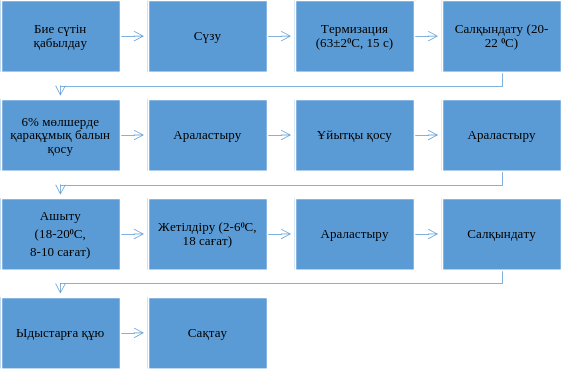
\includegraphics[width=0.6\textwidth]{assets/1105}
	\caption*{1-сурет - Қарақұмық балы қосылған қымыз өндіру технологиялық сызбасы}
\end{figure}

\begin{multicols}{2}
Қарақұмық балын қолдана отырып әзірленген қымыз технологиясы келесідей:
Бие сүті шикізаты ҚР СТ 1005-98 «Бие сүті» стандартында көрсетілген
көрсеткіштерге сәйкес қабылданады, дәке арқылы сүзіледі. Бие сүтін,
әрине, жылумен өңдемеген дұрыс, оның антиоксиданттық және
антибактериалды қасиеттерін жоғалтпау мақсатында, бірақ микробиологиялық
қауіпсіздігін қамтамасыз ету мақсатында 63±2°С температурада 15 секунд
термизация процесі жүргізіледі. Белгіленген жылумен өңдеу параметрлері
бие сүтінің бастапқы сапа көрсеткіштерінің толығымен сақталуын
қамтамасыз етеді. Қыздырылған сүт 20±2°С температурға дейін
салқындатылып оған 6\% мөлшерде қарақұмық балы қосылады, жақысылап
араластырып GENESIS компаниясының Lасtococcus lactis sp. lactis,
Laсtococcus lactis sp. cremoris, Laсtococcus lactis sp. lactis biovar.
diacetylactis, Leuconostoc mesenteroides sp.cremoris, Streptococcus
salivarius sp. thermophilus, Lactobacillus kefyr, Candida kefyr,
Sacchromuces unisporus күрделі құрамды ұйытқысын қосып араластырамыз,
18±2°С температурада, 6-8 сағат бойы ашытамыз, ашыту процесі аяқталғанан
кейін 2-6°С, 18 сағат бойы жетілдіру процесі жүзеге асырылады. Одан
кейін 1000 г пластик бутылкаларға құйылып, 4-5°С температурада
салқындатылып, 2-4°С температурада 36 сағат сақталады.

Қарақұмық балын дайындау. Қарқұмық балды қолданар алдында бал 40-50°С
дейін қызады, содан кейін 2 мм ұяшықтары бар електен сүзіледі.

Балдың түсін анықтау. Бал түтікке немесе түссіз шыны цилиндрге құйылады
(егер бал кристалданған болса, ол 40-45°С температурада су ваннасында
алдын ала ерітіледі). Балдың түсі күндізгі жарықта көзбен анықталады.
Әрі қарай балдың хош иісін анықтайды. Ол үшін шыны бюкске (стаканға)
30-40 г бал қойылады, қақпақпен жабылады және су ваннасында 40-45°С
температурада 10 минут қыздырылады. Бюкс ваннадан алынады, қақпақ
алынып, мұрын арқылы қысқа дем алынады.

Балдың дәмін анықтау. Балдың дәмін бағалау үшін оңтайлы температура 30°С
болып саналады, сондықтан зерттеу алдында сынақ су ваннасында
жылытылады.

Балдың консистенциясын анықтау. Консистенциясы шпательді балға батыру
арқылы анықталады, температурасы 20°С, шпатель алынып, балдың ағу сипаты
бағаланады. Содан кейін балды қымыз дайындауға қолданады.

Әзірленген жаңа қарақұмық балы қосылған қымыздың органолептикалық және
физико-химиялық көрсеткіштері анықталды. Нәтижелері 8-9 кестелерде
көрсетілген.
\end{multicols}

\begin{table}[H]
\caption*{8-кесте - Қарақұмық балы қосылған қымыздың органолептикалық көрсеткіштері}
\centering
\begin{tabular}{|l|p{0.4\textwidth}|}
\hline
Көрсеткіштер аталуы & Нәтижелер \\ \hline
Сыртқы түрі & мөлдір емес сұйықтық \\ \hline
Консистенциясы & Сұйық, біртекті газдалған аздап көбіктенетін, ақуыз үлпектерісіз және жинақталған май бөлшектері жоқ \\ \hline
Дәмі және иісі & Таза, сүт қышқылды қымыз үшін ерекше, дәмі мен иісі жоқ. Ашытқы дәміне рұқсат етіледі. Сәл балдың дәмі мен иісі бар \\ \hline
Түсі & Сүтті ақ, аз ғана кремді реңкі бар, бүкіл салмағы бойынша біркелкі \\ \hline
\end{tabular}
\end{table}

\begin{table}[H]
\caption*{9-кесте - Қарақұмық балы қосылған қымыздың физика-химиялық көрсеткіштері}
\centering
\begin{tabular}{|l|l|}
\hline
Көрсеткіштер аталуы & Нәтижелер \\ \hline
Қышқылдық, °Т, аспау керек & 80 \\ \hline
Майдың салмақтық үлесі, \% & 1,43 \\ \hline
Ақуыздың салмақтық үлесі, \% & 1,62 \\ \hline
Көмірсулардың салмақтық үлесі, \% & 8 \\ \hline
Энергетикалық құндылығы, ккал & 46,25 \\ \hline
\end{tabular}
\end{table}

\begin{multicols}{2}
{\bfseries Қорытынды.} Осылайша экперименттік және әдеби деректерге
жүргізілген зерттеулер нәтижесінде алғаш рет қарақұмық балы қосылған
қымызын алу мүмкіндігі дәлелденді. Қымызға қосылатын қарақұмық балының
оңтайлы дозасы таңдалынып, жаңа қымыз түрінің рецептурасы мен
технологиялық сұлбасы әзірленді.

Әзірленген жаңа қарақұмық балы қосылған қымыздың органолептикалық және
физико-химиялық көрсеткіштері анықталды.

Алынған қарақұмық балы қосылған қымыз бие сүтінен жасалған сүт
өнімдерінің ассортиментін кеңейтуге мүмкіндік береді.
\end{multicols}

\begin{center}
{\bfseries References}
\end{center}

\begin{noparindent}
1.Fotschki J, Szyc AM, Laparra JM, Markiewicz LH, Wróblewska B.
  Immune-modulating properties of horse milk administered to mice
  sensitized to cow milk // Journal of Dairy Science.- 2016.-Vol.
  99(12). - P. 9395-9404. DOI 10.3168/jds.2016-11499

2.Therese Uniacke-Lowe, Thom Huppertz, Patrick F.Fox. Equine milk
proteins: Chemistry, structure and

nutritional significance //
  International Dairy Journal.-2010.-Vol. 20(9). -P.609-629. DOI
  
  10.1016/j.idairyj.2010.02.007

3.3.Salimei, Elisabetta \& Park, Young. Mare milk. // In book: Handbook
  of Milk of Non-Bovine Mammals. - 2017.- P.369-408. DOI
  10.1002/9781119110316.ch5

4.Malacarne M., Martuzzi F., Summer A., Mariani P. Protein and fat
  composition of mare's milk: some nutritional remarks with reference to
  human and cow's milk // International Dairy Journal.- 2002.-Vol.
  12(11). -P. 869-877. DOI 10.1016/S0958-6946(02)00120-6

5.Doreau M., Martin W. -Rosset. Animals that Produce Dairy Foods
  \textbar{} Horse // Encyclopedia of Dairy Sciences.- 2011. - P.
  358-364. DOI 10.1016/B978-0-12-374407-4.00040-6

6.Salimei E., Fantuz F. Horse and donkey milk. // In book: Milk and
  dairy products in human nutrition: production, composition and health.
  -2013. -P. 594-613 DOI 10.1002/9781118534168.ch27

7.Markiewicz-Kęszycka M., Wójtowski J., Czyżak-Runowska G., Kuczyńska
B., Puppel K., Krzyżewski J.,

Strzałkowska N., Jóźwik A., Bagnicka E.
  Influence of stage of lactation and year season on composition of
  mares\textquotesingle{} colostrum and milk and method and time of
  storage on vitamin C content in mares\textquotesingle{} milk //
  Journal of the Science of Food and Agriculture. -- Vol. 95. -- Iss.
  11. -P: 2279-2286. DOI 10.1002/jsfa.6947

8.Clayes W.L., Verraes C., Cardoen S., De Block J., Huyghebaert A., Raes
  K. Consumption of raw or heated milk from different species: An
  evaluation of the nutritional and potential health benefits / Food
  Control. -- 2014. -- Vol. 42. --P. 188-201. DOI
  10.1016/j.foodcont.2014.01.045

9.L. Businco, P.G. Giampietro, P. Lucenti, F. Lucaroni, C. Pini, G. Di
  Felice, P. Iacovacci, C. Curadi, M. Orlandi. Allergenicity of mare's
  milk in children with cow's milk allergy / Journal of Allergy and
  Clinical Immunology. -- 2000. -- Vol. 105. -- Iss. 5. -- P. 1031-1034.
  DOI 10.1067/mai.2000.106377

10.Haddad I., Mozzon M., Strabbioli R., Frega N.G.. A comparative study
  of the composition of triacylglycerol molecular species in equine and
  human milks / Dairy Science and Technology. -- 2012. -- Volume 92. --
  P. 37-56. DOI 10.1007/s13594-011-0042-5

11.Park Y.W. Bioactive Components in Milk and Dairy Products. John Wiley
  \& Sons. -- 2009. --440p. DOI 10.1002/9780813821504

12.Curadi M.C., Giampietro P.G., Lucenti P., Orlandi M. Use of mare milk
  in pediatric allergology / Proc. ASPA Congr. Rec. Prog. Anim. Prod.
  Sci., Associazione Scientifica di Produzione Animale. -- Italy, 2001.,
  -- P. 647-649.

13.Haddad, I., Mozzon, M., Strabbioli, R., Frega, N.G. A comparative
  study of the composition of triacylglycerol molecular species in
  equine and human milks / Dairy Science and Technology. - 2012. - Vol.
  92. - P: 37-56. DOI 10.1007/s13594-011-0042-5
\end{noparindent}

\emph{{\bfseries Авторлар туралы мәліметтер}}

\begin{noparindent}{2}
Диханбаева Ф.Т. - техника ғылымдарының докторы, Алматы технологиялық
университеті, Алматы, Қазақстан, e-mail: fatima6363@mail.ru;

Есиркеп Г.Е. - техника ғылымдарының кандидаты, Қ. Құлажанов атындағы
Қазақ технология және бизнес университеті, Астана, Қазақстан, e-mail:
milana.anar@mail.ru;

Жунусова Г.С. - техника ғылымдарының кандидаты, Қ. Құлажанов атындағы
Қазақ технология және бизнес университеті, Астана, Қазақстан, e-mail:
gulzat\_7@mail.ru;

Нармандах Ж. - магистр, оқытушы, Қ. Құлажанов атындағы Қазақ технология
және бизнес университеті, Астана, Қазақстан, e-mail:
zhupar10\_89@mail.ru;

Калемшарив Б. - докторант, С. Сейфуллин атындағы Қазақ агротехникалық
зерттеу университеті, Астана, Қазақстан, e-mail: begjan.ae@gmail.com.
\end{noparindent}

\emph{{\bfseries Information about the authors}}

\begin{noparindent}
Dikhanbaeyva F.T. - Doctor of Technical Sciences, Almaty Technology
University, Almaty, Kazakhstan, e-mail: fatima6363@mail.ru;

Esirkep G.E. - Candidate of Technical Sciences, Kazakh University of
Technology and Business named after Kulajanov, Astana, Kazakhstan,
e-mail: milana.anar@mail.ru;

Zhunusova G.S. - Candidate of Technical Sciences, Kazakh University of
Technology and Business named after Kulajanov, Astana, Kazakhstan,
e-mail: gulzat\_7@mail.ru;

Narmandakh Zh. - master teacher, Kazakh University of Technology and
Business named after Kulajanov, Astana, Kazakhstan, e-mail:
zhupar10\_89@mail.ru;

Kalemshariv B. - doctoral student, Kazakh Agrotechnical Research
University named after Seifullin, Astana, Kazakhstan, e-mail:
begjan.ae@gmail.com.
\end{noparindent}
